\documentclass{article}

\usepackage{graphicx}

\title{Problem9 Report}
\author{Qi Liu}
\date{\today}

\begin{document}

\maketitle

\section{Edge Detection}
We have implemented Roberts, Prewitt, Sobel, Marr-Hildreth and Canny edge detectors. The results are shown below.

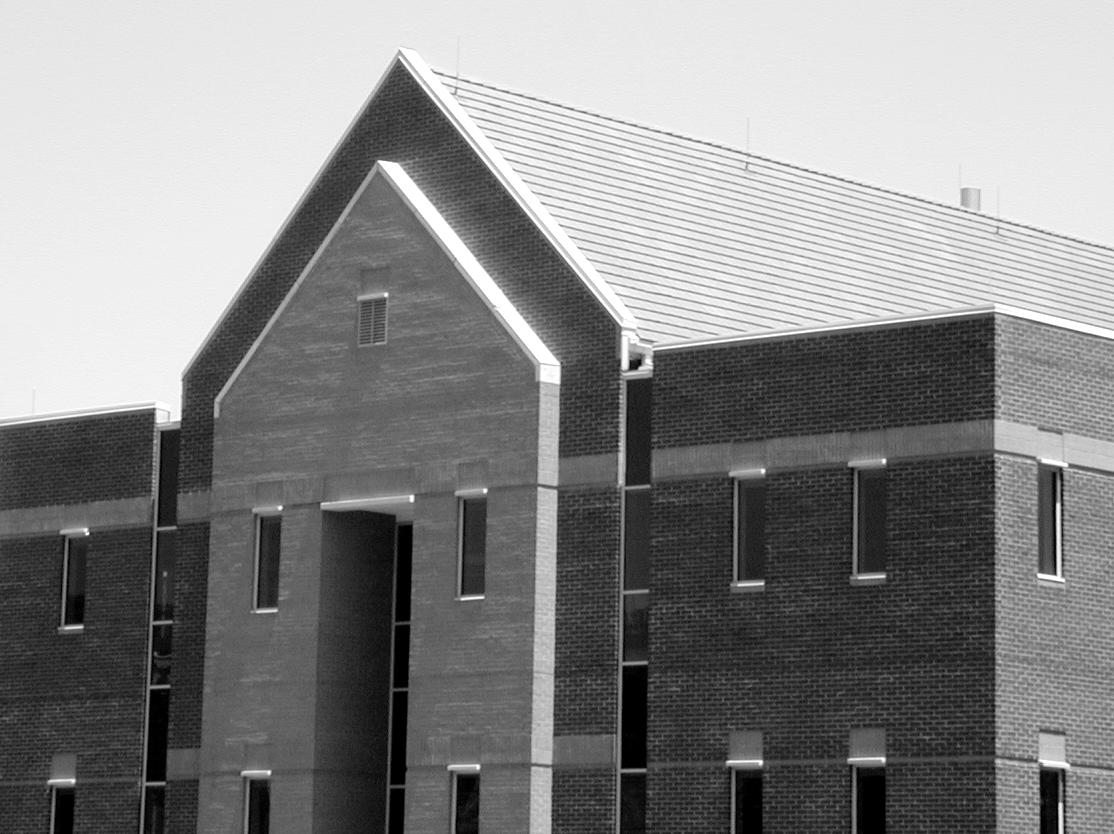
\includegraphics[width=0.33\textwidth]{../data/building.jpg}
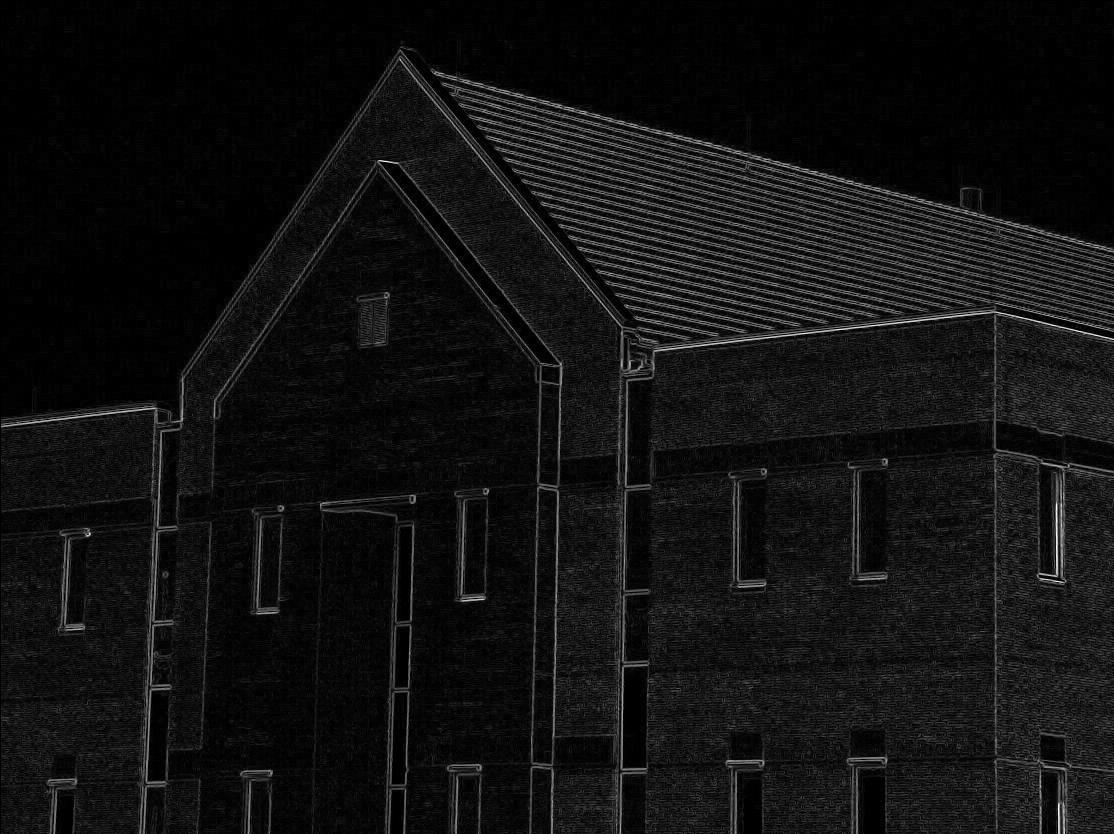
\includegraphics[width=0.33\textwidth]{../data/roberts_building.jpg}
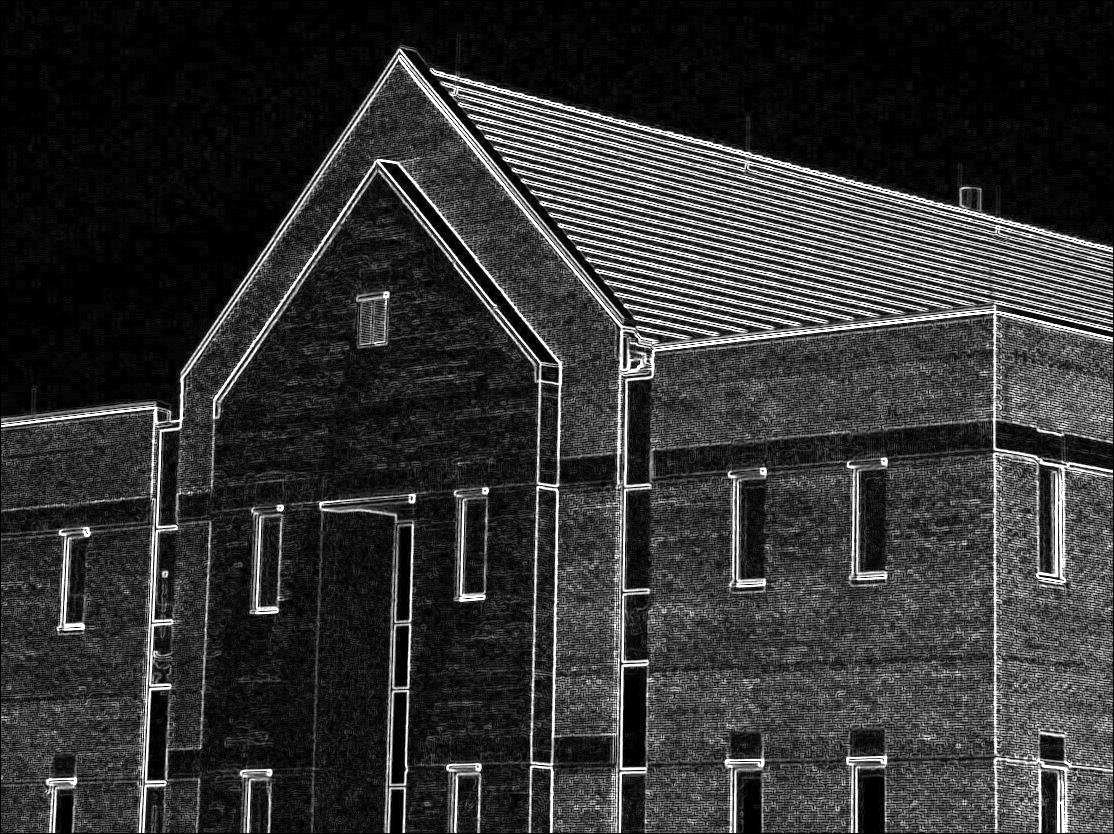
\includegraphics[width=0.33\textwidth]{../data/prewitt_building.jpg}

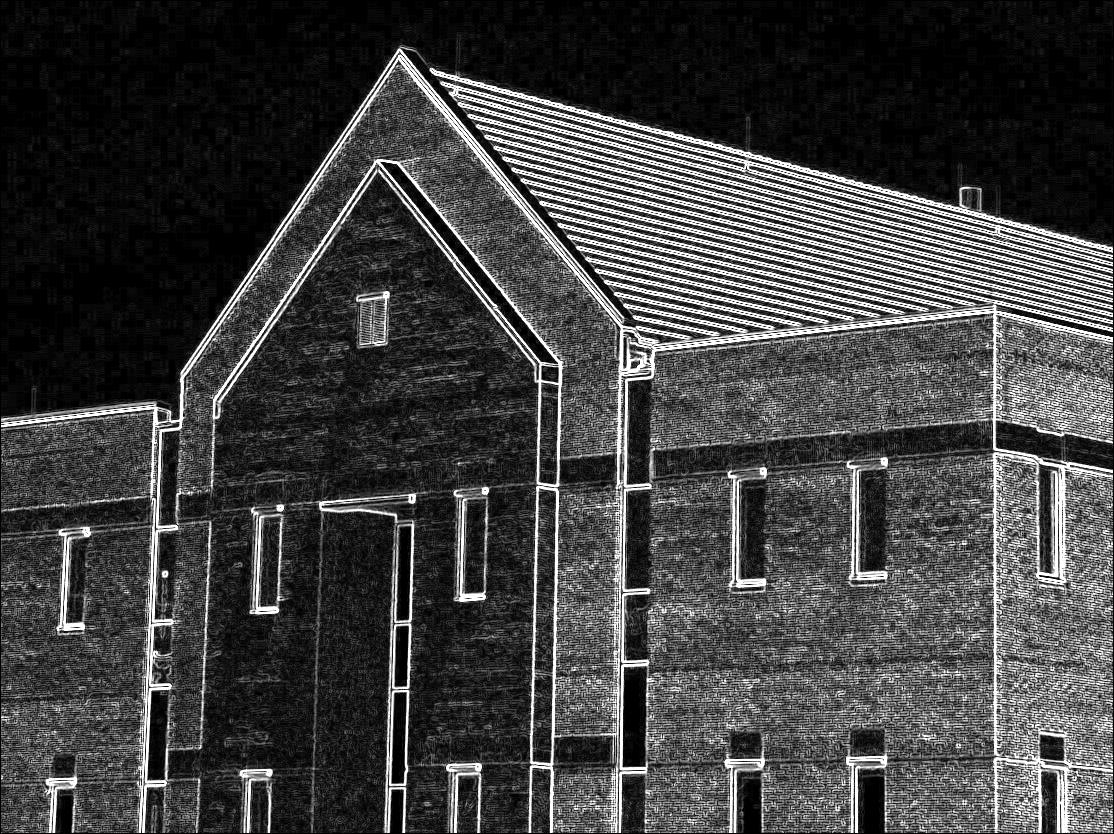
\includegraphics[width=0.33\textwidth]{../data/sobel_building.jpg}
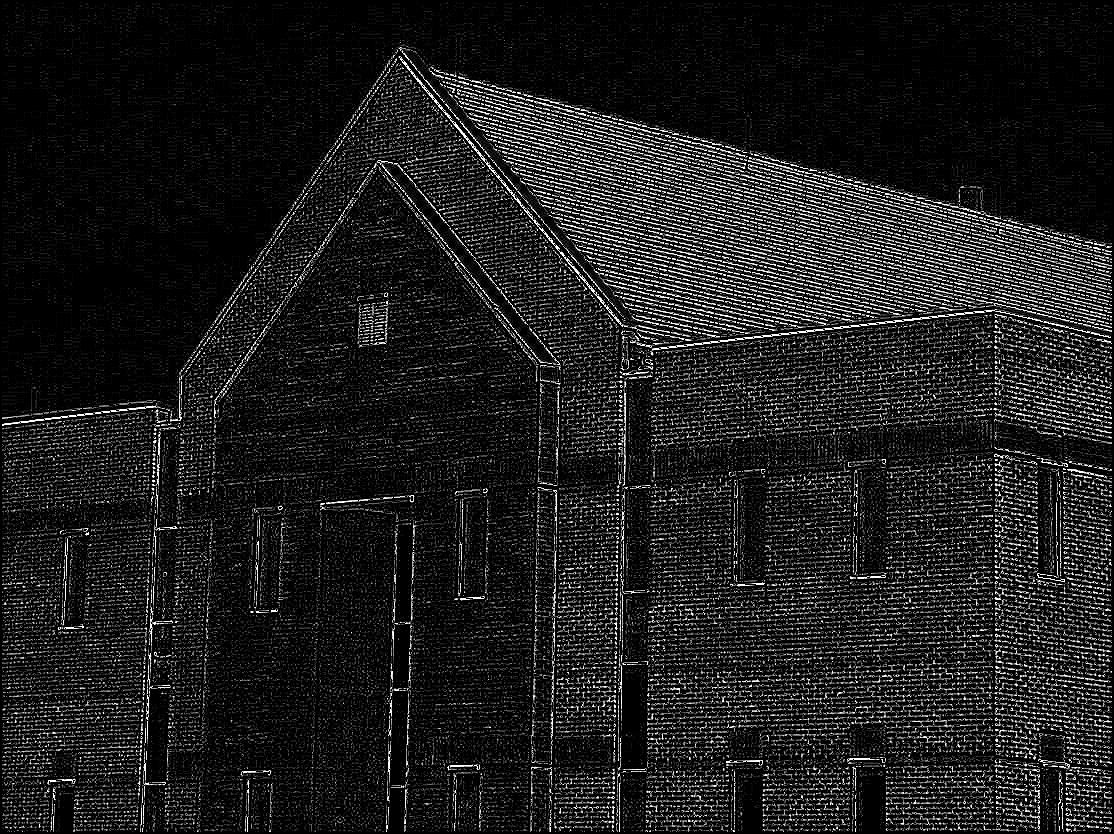
\includegraphics[width=0.33\textwidth]{../data/marr_hildreth_building.jpg}
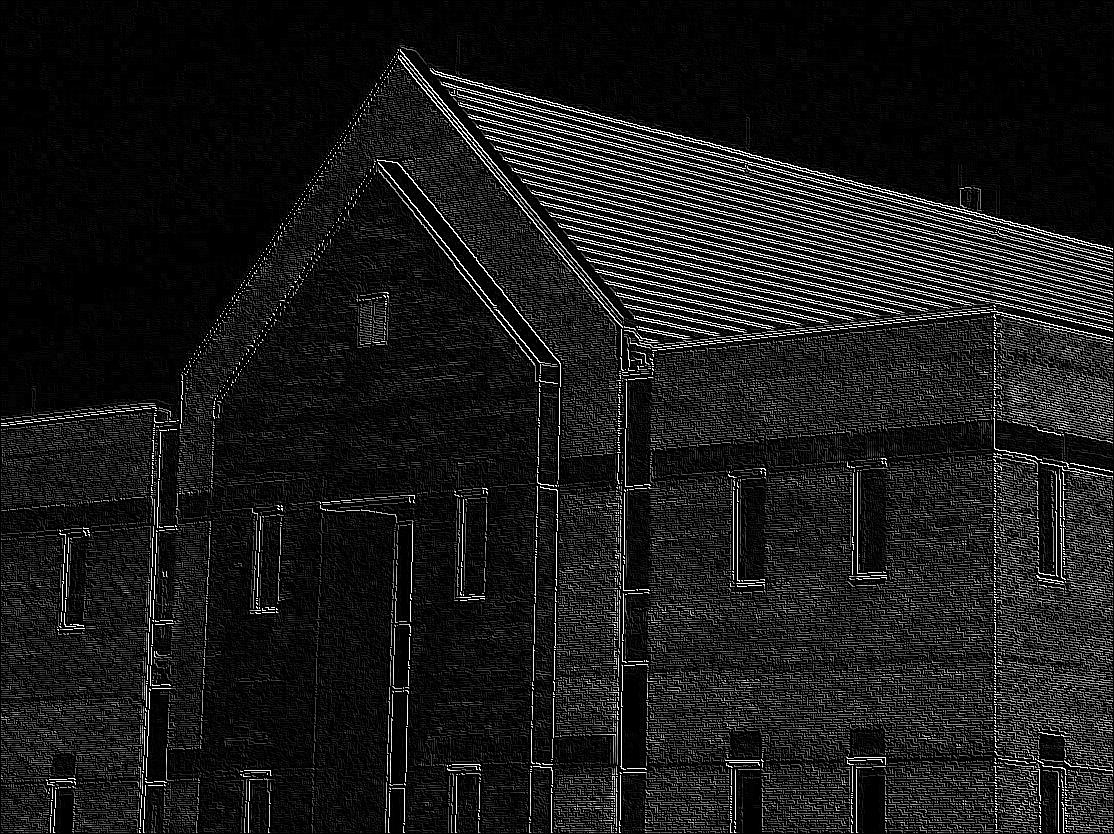
\includegraphics[width=0.33\textwidth]{../data/canny_building.jpg}

The first one is the original image. The second to the fourth are results of Roberts, Prewitt and Sobel by using the masks 
\begin{tabular}{|c|c|}
	\hline -1&0\\
	\hline 0&1\\
	\hline
\end{tabular}
\begin{tabular}{|c|c|}
	\hline 0&-1\\
	\hline 1&0\\
	\hline
\end{tabular},
\begin{tabular}{|c|c|c|}
	\hline -1&-1&-1\\
	\hline 0&0&0\\
	\hline 1&1&1\\
	\hline
\end{tabular}
\begin{tabular}{|c|c|c|}
	\hline -1&0&1\\
	\hline -1&0&1\\
	\hline -1&0&1\\
	\hline
\end{tabular} and
\begin{tabular}{|c|c|c|}
	\hline -1&-2&-1\\
	\hline 0&0&0\\
	\hline 1&2&1\\
	\hline
\end{tabular}
\begin{tabular}{|c|c|c|}
	\hline -1&0&1\\
	\hline -2&0&2\\
	\hline -1&0&1\\
	\hline
\end{tabular} respectively. We can see the edges in Prewitt and Sobel are more clear than Roberts but with more noises. The fifth image is the result of Marr-Hildreth, we use the mask $$\begin{tabular}{|c|c|c|c|c|}
\hline 0&0&-1&0&0\\
\hline 0&-1&-2&-1&0\\
\hline -1&-2&16&-2&-1\\
\hline 0&-1&-2&-1&0\\
\hline 0&0&-1&0&0\\
\hline
\end{tabular}$$ to filter the image first and than find the zero crossing to get the result. We can see the edges of bricks are more clear than previous images but the edges of roof are a little blurred. The sixth image is the result of Canny. We use Prewitt mask to calculate the gradient in Canny algorithm. We can see the result is good, almost every edge is clear.

\section{Thresholding}

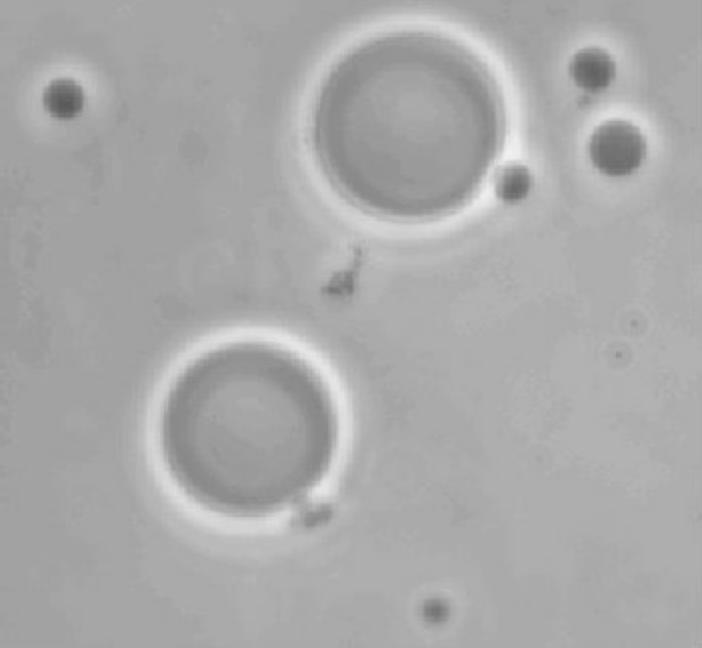
\includegraphics[width=0.33\textwidth]{../data/polymersomes.jpg}

\includegraphics[width=0.33\textwidth]{../data/global_polymersomes.jpg}
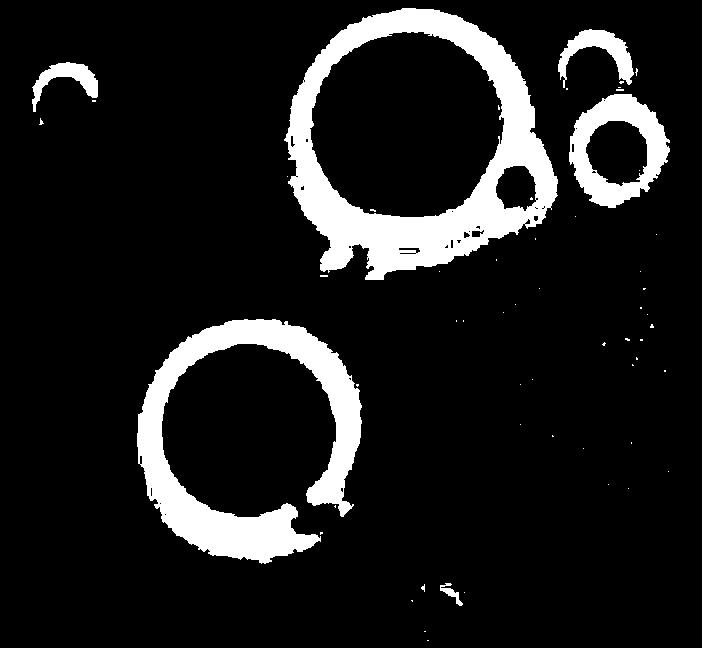
\includegraphics[width=0.33\textwidth]{../data/otsu_polymersomes.jpg}

The first image is the original one. The second image is the result of global thresholding and the threshold is 169. We can see it is not good due to background and object are not distinguishable. The third image is the result of Otsu thresholding and the threshold is 181. We can see a better result than the second one.

\end{document}